\Chapter{A tűz megjelenítése}

% TODO: Összeszedni az eddigi eredményeket a tűz megjelenítésével kapcsolatban!

\section{Megvalósítás a fontosabb játékmotorokban}

A háromdimenziós játékok felemelkedése az 1990-es években kezdődött. Az első játékmotorok az id Software fejlesztőinek köszönhetőek. Ahelyett, hogy minden játékot egyenként az alapoktól kezdve építettek volna fel, más fejlesztők által készített modulokat használtak. Megtervezték a saját grafikájukat, karaktereiket, fegyvereiket és pályáikat, melyek lényegében a játék tartalmát nyújtották. Így már szét lehetett választani a játékspecifikus szabályokat és adatokat olyan alap koncepcióktól, mint például az ütközésvizsgálat. Ennek köszönhetően a fejlesztői csapatokat lehetett bővíteni, hiszen egyszerre több modulon is lehetett párhuzamosan, egymástól függetlenül dolgozni. Ez lehetővé tette továbbá, hogy a fejlesztők külön területekre specializálódjanak \cite{wikiGameEngine}.

A specializáció egy jellegzetes iránya a játékokban a tűzhöz kapcsolódó jelenségek modellezése. A korábbi, kétdimenziós játékokban csak sprite (kétdimenziós bitmap) alapú tüzekkel találkozhatunk. Az id tech 1 motor sem kivétel, habár hármodimenziósnak tűnnek a vele készült játékok (például Doom I, Doom II), a benne lévő objektumok szintén sprite-ok, melyek mindig a néző felé fordulnak. Az ilyen játékmotorokat 2.5 dimenziós motoroknak is nevezhetjük. 

%Sprite tűz:
%1993 id tech 1/doom engine https://en.wikipedia.org/wiki/Doom_engine +  https://doomwiki.org/wiki/Doom_rendering_engine 
% Doom II: Hell on Earth (id tech 1 ez is)

\subsection{Quake engine 1996}

% MDL format: http://fabiensanglard.net/quakeSource/quakeSourceRendition.php
% torch animation http://media.moddb.com/images/members/1/240/239733/qv1.gif

A Quake motor 1996-ban készült el a Quake számítógépes játék számára. Az id tech 1 motorral ellentétben ez már igazi háromdimenziós motor, azaz háromdimenziós adatokat felhasználva állítja elő a kétdimenziós képet. A megjelenítés valós időben történik. A játékban egyaránt használtak fénytérképeket (lightmap) és 3D-s fényforrásokat is. Előbbi segítségével a statikus objektumok fényét lehetett az objektumokra égetni, ezzel rövidítve a kirajzolási időt, utóbbi pedig a dinamikus objektumok fényét adta \cite{wikiQuake}.

A játékban a fáklyák tüzét vizsgáltam. A tűz maga váltakozó modellek sorozatából állt, melyet MDL fájformátumban tároltak le. Ez a formátum lehetővé teszi a képkockáról képkockára való animáció tárolását. Egy .mdl fájl jellemzői az alábbiak:
\begin{itemize} 
\item a modell geimetriai adatai (háromszögekben),
\item textúra adatok,
\item képkockáról-képkockára való animáció.
\end{itemize} 
Egy MDL fájlban több textúra is lehet. Minden képkockához külön-külön hozzá lehet rendelni egyebek mellett, hogy mely csúcsok szerepelnek benne. A formátum lehetővé teszi egy befoglaló gömb megadását is, mely ütközésvizsgálatok esetén lehet fontos, ám ezt nem kötelező megadni benne \cite{MDLformat}. 

% http://tfc.duke.free.fr/coding/mdl-specs-en.html

Tehát a tűznek semmiféle külön fizikai modellezéséről sincs szó (legalábbis valós időben). Előre meg van határozva a mozgása képkockákra lebontva. A fáklyák kaphattak pislákoló fényt, ám ez rendkívül lassította a kirajzolást, így többnyire csak olyan helyen lehetett alkalmazni ahol kevés felületet világított meg. Mint az \aref{fig:quakeTorch}. ábrán is látszik. A tűz lángjain nem lehet átlátni, illetve füstképződés sincs. Az interneten fellelhető videók alapján arra a következtetésre jutottam, hogy a lánggal való ütközés nincs külön vizsgálva. Azt is sikerült megfigyelnem, hogy amennyiben egyszerre több helyen is meg van jelenítve a láng modellje, mindenhol ugyanaz a modell látszik. Ebből arra lehet következtetni, hogy nem volt több külön betöltött példány, csupán egyetlen egy láng objektum, melyet egyszerre több helyen is megjelenítettek (\ref{fig:quakeTorch}. ábra). Ennek oka a korabeli számítógépek korlátozott memóriájára vezethető vissza. A játék OpenGL-es portjában a gyorsítás érdekében a modelleket DisplayList-ekbe töltötték be (\texttt{gl\_mesh.c}).

\begin{figure}[h]
\centering
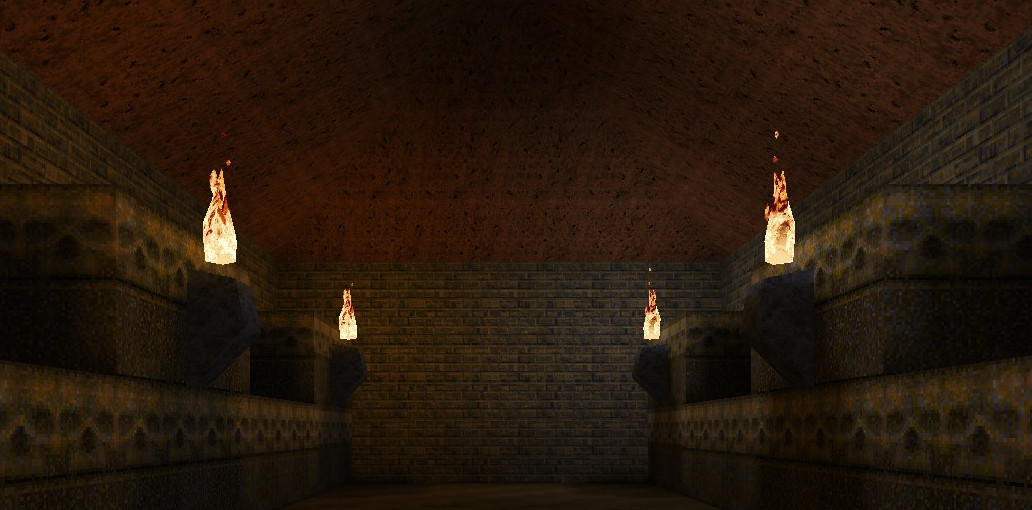
\includegraphics[width=\textwidth]{kepek/quake_torches2.jpg}
\caption{Ugyanazon modell megjelenítése egyszerre több helyen a Quake motorban}
\label{fig:quakeTorch}
\end{figure}

\subsection{Quake II (id tech 2) engine}

% slow-mo explosion video: https://www.youtube.com/watch?v=L66vRF5VOVM
% md2 format: http://tfc.duke.free.fr/coding/md2-specs-en.html

A Quake motor utódjaként született meg a Quake 2, avagy az id tech 2 motor, melyen elsőként az 1997-ben megjelent Quake II játék alapult. Ez a motor már a szoftveres megjelenítés mellett az OpenGL segítségével a megjelenítés hardveres gyorsítását is támogatta. Utóbbinak köszönhetően színezett fény effektusok használata, illetve bilineáris textúra szűrés (4 pont közötti interpoláció) is lehetővé vált. Fénytérképeket itt is használtak, ám ezek már dinamikusan változtathatóak voltak \cite{wikiQuake2, fsQuake2}. Tűz megjelenítés szempontjából a Quake II játékot vizsgáltam, melyben fáklya nem volt, viszont robbanás effekt igen (\ref{fig:quake2explosion}. ábra).

\begin{figure}[h]
\centering
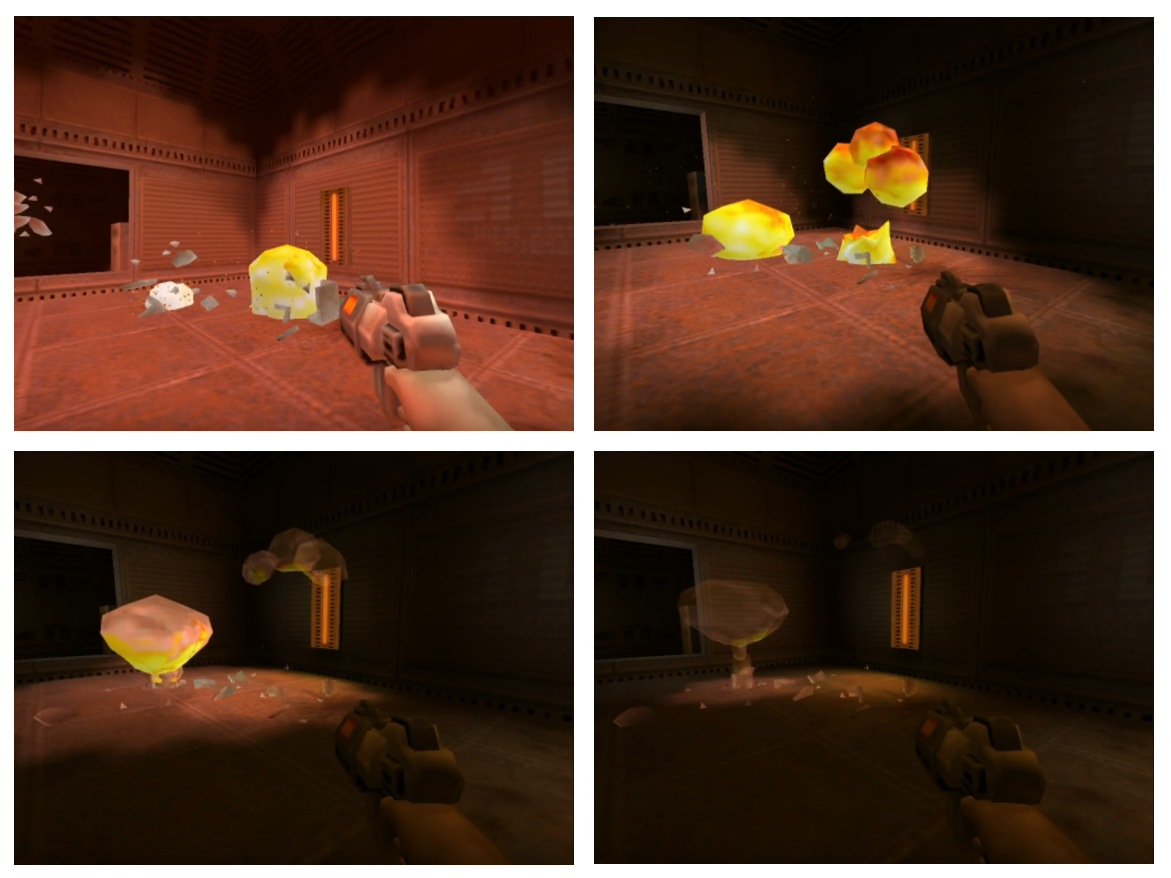
\includegraphics[width=\textwidth]{kepek/quake2explosion9.png}
\caption{A robbanás folyamatának néhány szemléltető állomása a Quake II-ben}
\label{fig:quake2explosion}
\end{figure}

Az első Quake motorhoz hasonlóan a robbanás folyamata itt is előre meg van határozva képkockáról képkockára. Ebben az esetben az ilyen animált modelleket \texttt{md2} kiterjesztésű fájlokban tárolták le melyek tartalmazták:
\begin{itemize} 
\item a modell geimetriai adatait (háromszögekben),
\item a képkockáról képkockára való animációt,
\item a strukturált adatokat, melyek a \texttt{GL\_TRIANGLE\_FAN} és \texttt{GL\_TRIANGLE\_STRIP} primitívek rajzolásához szükségesek OpenGL-ben.
\end{itemize} 
Az MDL formátummal ellentétben a model textúrája egy külön fájlban foglal helyet. Egy MD2 modellnek egyszerre csak 1 textúrája lehet \cite{MD2format}.

Fizikai modellről tehát valós időben itt sem beszélhetünk. A Quake-hez képest viszont sokkal finomabb az animáció, mely arra enged következtetni, hogy a frame-ek közötti állapotokat interpolálták. Így minél nagyobb a frame-rate, annál folyékonyabb a mozgás. A robbanásokhoz tartozik dinamikus fény is. Mivel a robbanások bekövetkezése nem egy időben zajlik, egyszerre több külön modellt is meg kell jeleníteni különböző állapotokban, viszont a maximális robbanások száma egy időben 32-re van korlátozva (\texttt{cl\_tent.c}). A robbanás modelljén kezdetben nem lehet átlátni, de amint kibontakozik a lángcsóva, áttetszővé válik a modell és beszürkül, ami a robbanás füstjét kívánja ábrázolni. Ütközésvizsgálat nincs a lángcsóvákra, viszont a játékost visszalöki a robbanás, ha az a közelében történik. 

\subsection{id tech 3 engine}

Az id tech 2 motoron alapult az id Software következő motorja, az id tech 3. Elsőként a Quake III Arena játékban debütált 1999-ben. Elődjeivel ellentétben ebben már nem volt szoftveres renderelés, tehát a futtatásához OpenGL kompatibilis grafikai gyorsítóra volt szükség, ami abban az időben nem volt jellemző a játékmotorokra \cite{wikiQuake3}.

% TODO: Érdemes lenne az Unreal-ról, mint akkor kompetítorról is szót ejteni!

Az id tech 2-ből ismert fénytérképen alapuló megvilágítást és multitextúrázást itt is használták. A motor egyik újítása a shader rendszer, melyet az OpenGL fix funkciójú csővezetékére (\textit{fixed function pipeline}) építettek. A fixed function pipeline az OpenGL régebbi verzióiban fellelhető konfigurálható feldolgozási állapotok gyűjteményére utal. Ezeket váltották fel a modern OpenGL shader-ei később \cite{fsQuake3}.

Az id tech 3 árnyalói viszont szöveges szkript fájlok formájában adottak, melyek egy adott felület kinézetét, tulajdonságait és viselkedését írják le. Az előrhető dokumentációban a módosított textúra szettek is fel vannak sorolva. Különféle kulcsszavak segítségével vannak elkülönítve a fizikai tulajdonságokat befolyásoló paraméterek és a kinézetre vonatkozó jellemzők. Egyszerre több shader effekt is tartozhat egy objektumhoz, de egy-egy shader használata is nagy számítási igényt von maga után, ugyanis a világnak azon részét befolyásolhatja, ezért újra kell rajzolni \cite{quake3shaderManual}.

A tűz effektek szempontjából fontos kulcsszavak például az alábbiak \cite{quake3shaderManual}.
\begin{itemize} 
\item
\texttt{DeformVertexes autosprite2}: Segítségével bármely (2 háromszögből álló) téglalap felület billboard-ként fog funkcionálni, anélkül, hogy erre külön objektumot hoznánk létre. Ez annyit tesz, hogy a sprite, amin a textúra van, mindig a nézőpontnak megfelelően fordul a hosszabbik tengelye mentén. Ez a funkció éppen megfelelő egy tűzoszlop megjelenítéséhez.
\item
\texttt{AnimMap <frequency> <texture1> ... <texture8>}: Olyan felületet határoz meg, mely a megadott textúrák sorozatának segítségével animálható. A \texttt{<frequency>} megadja, hogy 1 másodpercen belül hányszor játszódjon le a sorozat. A \texttt{<texture1> ... <texture8>} segítségével adhatjuk meg a felhasználni kívánt textúrák nevét, vagy elérési útvonalait. Nem kötelező mind a nyolcat megadni. Ha például megadunk 4 textúrát 0.25-ös frekvenciával, akkor egy 4 másodperces animációt kapunk, melyben minden textúrát 1 másodpercig látni. 
\item
\texttt{blendFunc}: Segítségével megmondhatjuk a motornak, hogy hogyan vegyítse a különbőző grafikus rétegeket (átlátszóság esetén).
\item
\texttt{rgbGen <func>}: Segítségével különféle pulzáló effekteket lehet készíteni. Ezeket úgy valósítja meg, hogy a megadott funkciónak megfelelően a csúcspontok (vertex) színét 2 érték között változtatja.
\end{itemize}

A Quake III Arena játékot vettem alapul a tűz effektek vizsgálatánál (habár a \ref{fig:quake3fire}. ábrán látható felvételeket a játék \textit{QuakeJs} portjában készítettem). Ebben robbanás és fáklya animáció is fellelhető volt. A két effekt megjelenítési módja közt csupán annyi különbséget véltem felfedezni, hogy amíg a robbanást billboard alapon ábrázolták, addig a fáklyák tüze csupán két, egymásra merőleges animált sprite-ból áll, mely jól megfigyelhető a \ref{fig:quake3fire}. ábrán. Ezen megoldásokból kifolyólag persze szükség van átlászóság használatára is. Füstöt nem kaptak az effektek, de fényt bocsátanak ki. Utóbbi megvalósítása a fáklyák esetén lehetséges statikus fénytérképekkel, de a robbanásokhoz dinamikusan változó fénytérképekre van szükség. Ütközésvizsgálat nem tartozik hozzájuk. Az effektek animációja tehát ismét egy előre meghatározott képsoron alapul. Az elődökhöz képest sokkal valósághűbbnek hatnak, pedig lényegesen kevesebb csúcspont felhasználásával lettek megvalósítva.

% TODO: Rocket kapcsán lehet írni a füstről is néhány dolgot.

\begin{figure}[h]
\centering
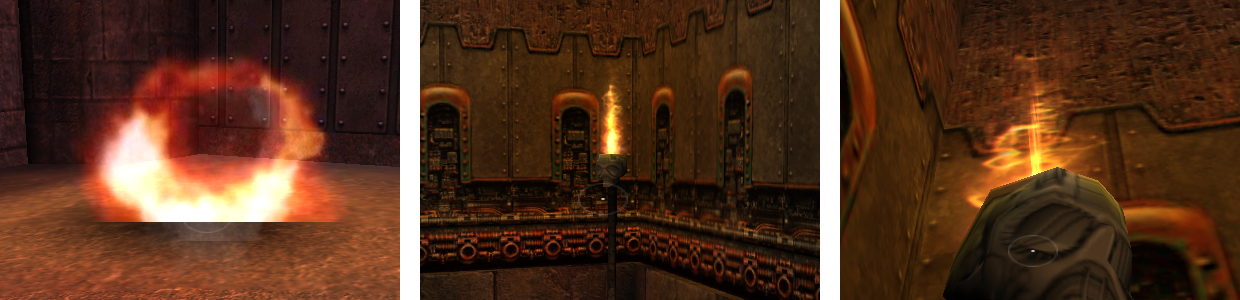
\includegraphics[width=\textwidth]{kepek/quake3fire.png}
\caption{A robbanás és a fáklya tüzének megjelenítése a Quake III Arena játékban}
\label{fig:quake3fire}
\end{figure}

%\subsection{ id tech 4 engine 2004}
%Az id tech 3 nagy részét átírva született meg az id tech 4 engine, mely 2004-ben mutatkozott be a nagyközönség előtt a Doom II játék motorjaként.
%Nincs elég anyag :(

% TODO: Return to Castle Wolfeinsten-ben vannak lángoló zombik! :) ..és lángszóró.

\subsection{Unreal engine 4}

Az Epic Games által készített Unreal engine 4 motorot elsőként 2012-ben mutatták be. A motor legfőbb újítása a valós idejű globális megvilágítás megvalósítása volt. Rengeteg új fejlesztői funkcióval látták el, mellyel lényegesen csökkentették a fejlesztési időt. Ilyen például a lehetőség, hogy a motor futása közben frissíthessük a kódot. Az új vizuális szkript rendszernek köszönhetően C++ kód írása nélkül is gyorsan fejleszthetővé vált a játék logikai része. Fejlesztés közben a változtatások azonnal megjeleníthetőek és tesztelhetőek. Eredményképpen egy olyan motor született, mely csökkenti a fejlesztési iterációk idejét, illetve szűkíti az űrt a műszaki művészek, tervezők és programozók között. A motort 2014-ben forráskóddal együtt ingyenesen elérhetővé tették tanulóknak, és egyetemi hallgatóknak egyaránt \cite{wikUE4}.

A motorhoz részletes dokumentáció és jónéhány mintaprogram is tartozik. Az id tech 3 óta rengeteget fejlődtek a graifkai gyorsító hardverek, így a modern játékmotorokban modell vagy képsorozatok helyett sokkal elterjedtebbek a részkecske rendszeren alapuló tűz effektek. Ezekben már fellelhető némi fizikai modellezés is, de a tűz valóságosságát számos apró trükk segítségével érik el. Mivel a részecskék mozgása nincs előre megadva, csupán néhány szabály van a sebességükre, irányukra és élettartamukra vonatkozóan, némi véletlenszerűséggel fűszerezve, a renderelt tűzben nem lehet ismétlődésekre lelni, mely rendkívül sokat javít az effekt valószerűségén. Az Unreal engine dokumentációjában megtalálható egy minta program, melyben egy fáklya tüzét jelenítik meg (\ref{fig:UE4fire}. ábra).

A fáklya tüze részecskerendszeren alapul, és a környezetét is megvilágítja. Az utóbbira létezik egy külön fény modul a motorban, mely a részecskék helyére dinamikus fényforrásokat helyez el. A fény világossága, színe és hatótávolságának sugara paraméterezhető. A részecskerendszerhez implementáltak \textit{levels of detail} (LOD) megoldást is. Nagy távolságokból a rendszer bizonyos részei túl kicsivé válhatnak ahhoz hogy kirajzolásra kerüljenek, ám ezeket továbbra is fel kellene dolgozni minden egyes képkockához, mely felesleges erőforrás felhasználást eredményez. Ennek elkerülése érdekében a távolság függvényében a részecskerendszer leegyszerűsíthető, bizonyos komponensei kikapcsolhatóak. A látványt nem rontják, viszont rengeteg processzor időt lehet megspórolni egy-egy ilyen megoldással \cite{UEngineFireExample}.

A valószerűség érdekében egy másik részecskerendszer segítségével izzó parázsdarabkák is felszállnak a tűz lángjaiból. Ezek turbulens hatást keltve mozognak, amit a lokális vektormező segítségével értek el, mely szintén a motor részét képezi. A mező háromdimenziós vektorait folyadék szimulációs adatokból nyerték ki, ezért olyan meggyőző a részecskék mozgása. Ahogy a részecskék haladnak a mezőben, a tér bizonyos pontjaiban az ott elhelyezkedő vektorok hatással lehetnek a sebességükre. A vektormező forgatásához a \textit{VF Rotation Rate} modult használták. Mivel a vektormező maga is turbulens hatást gyakorol a részecskékre, de maga a vektormező is mozgásban van, az eredmény egy rendkívül véletlenszerű, természetes turbulens hatást keltő részecske mozgás \cite{UEngineFireExample}.

A \ref{fig:UE4fire}. ábrán jól látható, hogy a lángok áttetszőek, és habár ebben a mintaprogramban füst nem is tartozik hozzá, hasonló elven egy másik emitter segítségével azt is meg lehetne valósítani. Ütközéstvizsgálat viszont nem tartozik hozzá.

\begin{figure}[h]
\centering
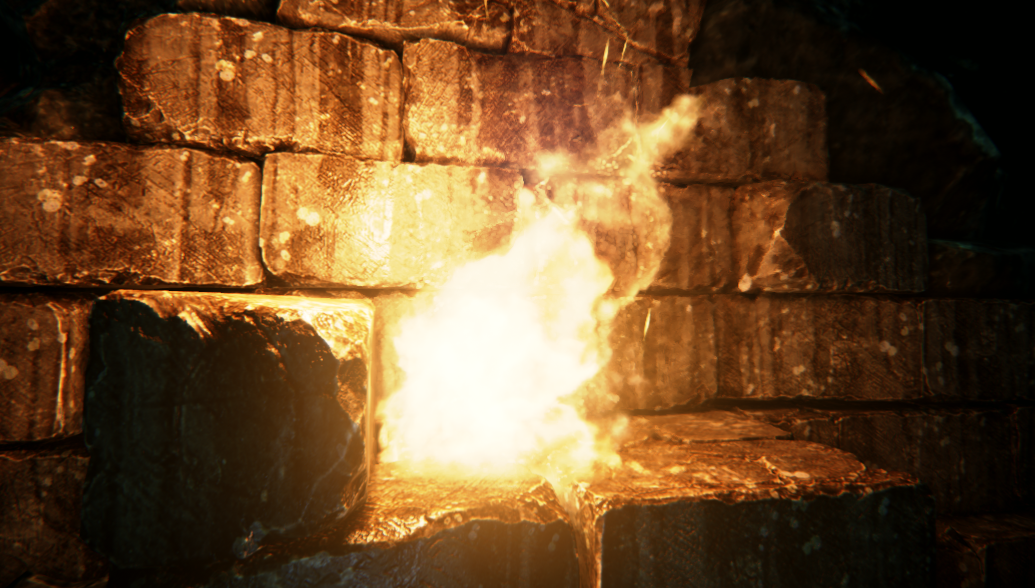
\includegraphics[width=\textwidth]{kepek/UE4flame.png}
\caption{Az Unreal engine 4 tűz effektje mely a dokumentáció alapján került megvalósításra \cite{UEngineFireExample}}
\label{fig:UE4fire}
\end{figure}

%\subsection{CRYENGINE 5.4 2017}
% 2017 CRYENGINE 5.4.0 https://github.com/CRYTEK/CRYENGINE



% Not open source:
% 1998 Unreal engine 1 
% 2002 Unreal engine 2
% 2004 CryEngine 1 https://github.com/AFCStudio/CRYENGINE-1 <- ez valami teljesen más
% 2007 Unreal engine 3
% 2012 Gamebryo 4.0  https://en.wikipedia.org/wiki/Gamebryo
% RenderWare https://en.wikipedia.org/wiki/RenderWare
% Fork_Particle https://en.wikipedia.org/wiki/Fork_Particle
% Source https://en.wikipedia.org/wiki/Source_(game_engine)
% Creation Engine https://en.wikipedia.org/wiki/Creation_Engine
% Crystal Tools https://en.wikipedia.org/wiki/Crystal_Tools
% Enigma Engine https://en.wikipedia.org/wiki/Enigma_Engine
% Frostbite https://en.wikipedia.org/wiki/Frostbite_(game_engine)
% GoldSrc https://en.wikipedia.org/wiki/GoldSrc
% IW engine https://en.wikipedia.org/wiki/IW_engine
% Jade https://en.wikipedia.org/wiki/Jade_(game_engine)
% RenderWare https://en.wikipedia.org/wiki/RenderWare
% Riot engine https://en.wikipedia.org/wiki/Riot_Engine
% RAGE https://en.wikipedia.org/wiki/Rockstar_Advanced_Game_Engine
% Vision https://en.wikipedia.org/wiki/Vision_(game_engine)#Games_using_Vision_Engine
% 2011 id tech 5 
% 2016 id tech 666

